\documentclass[tikz,border=2pt]{standalone}
\usepackage{amsmath}
\usepackage{pgfplots}
\pgfplotsset{compat=1.18}
\usetikzlibrary{arrows.meta}
\begin{document}
% Player 1's expected payoffs against q = sigma_2(L) in the 2x2 example: U gives 3q, D gives 2 - q;
% they tie at q = 1/2 with value 3/2. A third row B paying 1 earns 1 < 3/2 (equilibrium survives);
% a B paying 2 would earn 2 > 3/2 (the second condition fails).
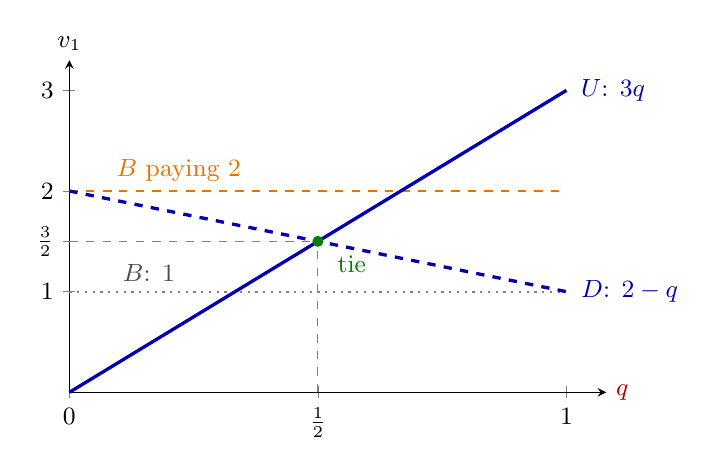
\begin{tikzpicture}[font=\small, >={Latex[length=2mm]}]
  \begin{axis}[
    width=8.4cm, height=5.8cm, axis lines=left,
    xmin=0, xmax=1.08, ymin=0, ymax=3.3,
    xtick={0,0.5,1}, xticklabels={$0$,$\tfrac12$,$1$},
    ytick={1,1.5,2,3}, yticklabels={$1$,$\tfrac32$,$2$,$3$},
    xlabel={$q$}, ylabel={$v_1$},
    xlabel style={red!70!black, anchor=west, at={(axis description cs:1,0)}},
    ylabel style={rotate=-90, anchor=south, at={(axis description cs:0,1)}},
    clip=false, every tick label/.append style={font=\small}]
    \addplot[gray, thick, dotted, domain=0:1] {1};
    \addplot[orange!90!black, thick, dashed, domain=0:1] {2};
    \addplot[blue!70!black, very thick, domain=0:1] {3*x};
    \addplot[blue!70!black, very thick, dashed, domain=0:1] {2-x};
    \draw[gray, thin, dashed] (axis cs:0.5,0) -- (axis cs:0.5,1.5);
    \draw[gray, thin, dashed] (axis cs:0,1.5) -- (axis cs:0.5,1.5);
    \fill[green!50!black] (axis cs:0.5,1.5) circle (2pt);
    \node[blue!70!black, anchor=west] at (axis cs:1.01,3) {$U$: $3q$};
    \node[blue!70!black, anchor=west] at (axis cs:1.01,1.0) {$D$: $2-q$};
    \node[gray!60!black, anchor=south] at (axis cs:0.16,1.0) {$B$: $1$};
    \node[orange!90!black, anchor=south] at (axis cs:0.22,2.0) {$B$ paying $2$};
    \node[green!50!black, anchor=north west] at (axis cs:0.52,1.45) {tie};
  \end{axis}
\end{tikzpicture}
\end{document}
